    \chapter{Methods}\label{cha:met}

    The methods utilized in this work are presented in the following chapter. Bayesian analysis and decision theory are introduced. Focus is laid on Bayesian inference, estimation of uncertain values and the use of loss functions in this context. These methods are incorporated in computational modeling of structural geological settings by programming in a python 3 environment. Central tools for model construction and conduction of the statistical evaluation are GeMpy and PyMC 2 in particular. These are also presented in this chapter.
    
        \section{Bayesian analysis and decision theory}\label{sec:bayes}
	    As implied by the name, the problems and reasoning behind decision-making are examined in the field of decision theory \citep{berger2013stat}. Such decision problems are commonly influenced by parameters that are uncertain. In statistical decision theory, available statistical knowledge is used to gain information on the nature of these uncertainties. (Such uncertain parameters can be considered as numerical quantities.) In order to find the best decision to a problem, it is possible to combine sample information with other aspects such as the possible consequences of decision-making and the availability of prior information on our uncertainties. Decision consequences are expressed as gains in economic decision theory and as losses, which equal negative gains, in statistics. Prior information might be given for example based on experience from previous similar problems or from expert knowledge (see Batvold and Begg). The approach of utilizing priors is known as Bayesian analysis, which is explained in the following \citep{berger2013stat}. (It goes well with decision theory.)
	    
	    \subsection{Basic elements}
	    First, some basic elements are to be defined. The unknown (uncertain) quantity influencing decision-making is usually denominated as the state of nature $\theta$ \citep{berger2013stat}. Given statistical information on $\theta$ in the form of probability distributions, $\theta$ is called the parameter. 
	    Decisions are also referred to as actions $a$.
	    The outcome of statistical tests in form of information or statistical evidence is denoted as $X$.	    
	    Loss is defined as $L(\theta,a)$, so $L(\theta_1,a_1)$ is the actual loss incurred when action $a_1$ is taken while the true state of nature is $\theta_1$ \citep{berger2013stat}. Loss, expected loss and loss functions are explained in detail further below.  
        
        \subsection{Bayesian inference}
        Bayesian inference is most importantly characterized by its preservation of uncertainty, in contrast to standard statistical inference \citep{davidson2015}. Probability is seen as a measure of belief for an event to occur. It has been argued by \cite{davidson2015}  that this Bayesian approach is intuitive and inherent in the natural human perspective. These beliefs can be assigned to individuals \citep{davidson2015}. Thus, different and even contradicting beliefs about the probability of an event might be held by different individuals, based on variations and disparities in the information available to each one individual \citep{davidson2015}.
        
        The initial belief or guess about an event A can be denoted as P(A) \citep{davidson2015}. This is used as the so-called prior probability on which Bayesian updating is based. The beliefs about the occurrence of an event are revalued in the presence of additional information, i.e. the observation of new evidence X. These observations are included as likelihoods P(X$|$A). This process of updating results in a posterior probability P(A$|$X) \citep{davidson2015}. It is important to note that the prior is not simply discarded but re-weighted by Bayesian updating. It was also pointed out by \citet{davidson2015} that by utilizing an uncertain prior, the potential for wrongfulness of the initial guess is already included. This means that Bayesian updating is about reducing uncertainty in a belief and reaching a guess that is less wrong \citep{davidson2015}.
        Bayesian updating is defined by and conducted via the following equation, called the Bayes' Theorem:
        
        \begin{equation}\label{eq:BayesTheorem}
        P(A|X) = \frac{P(X|A)P(A)}{P(X)}
        \propto P(X|A)P(A)
        \end{equation}
     
        -Law of Large Numbers!
                
        \subsection{Estimation}
        The resulting posterior distribution can be used to acquire point estimates for the true state of nature $\theta$. Common and simple examples for such estimators are the mode (i.e. the generalized maximum likelihood estimate), the mean and the median of a distribution \citep{berger2013stat}. The presentation of a point estimate should usually come with a measure for its estimation error. According to \citet{berger2013stat}, the posterior variance is most commonly used as an indication for estimate accuracy. However, it is argued by \citet{davidson2015} that by using pure accuracy metrics, while this technique is objective, it ignores the original intention of conducting the statistical inference in cases, in which payoffs of decisions are valued more than their accuracies. A more appropriate approach can be seen in the introduction of loss and the use of loss functions \citep{davidson2015}.
        
        \subsection{Expected loss and loss functions}\label{sec:loss} 
        Loss is a statistical measure of how bad an estimate is, i.e. how much is lost by making a certain decision. Gains are considered by statisticians as negative losses \citep{davidson2015}.
        The magnitude of an estimate's loss is defined by a loss function, which is a function of the estimate of the parameter and the true value of the parameter \citep{davidson2015}:
        
        \begin{equation}\label{eq:LossFunction}
        L(\theta,\hat{\theta}) = f(\theta,\hat{\theta})
        \end{equation}
        
        So, "how bad" a current estimate is, depends on the way a loss function weighs accuracy errors and returns respective losses. Two standard loss functions are the absolute-error and the squared-error loss function. Both are simple to understand and commonly used \citep{davidson2015}.
        
        As implied by its name, the absolute-error loss function returns loss as the absolute error, i.e. the difference between the estimate and the true parameter \citep{davidson2015}:
        
        \begin{equation}\label{eq:AbsLossFunction}
        L(\theta,\hat{\theta}) = |\theta - \hat{\theta}|
        \end{equation}        
        
        Accordingly, losses increasing linearly with the distance to the true value are returned for respective estimates. This means that all differences between relative errors are weighed equally, no matter whether they are found in the realm of relatively small or relatively large errors \citep{hennig2007}.
        
        Using the squared-error loss function returns losses that increase quadratically with distance of the estimator to the true parameter value \citep{davidson2015}:
        
        \begin{equation}\label{eq:SqrLossFunction}
        L(\theta,\hat{\theta}) = |\theta - \hat{\theta}|^2
        \end{equation}        
        
        This exponential growth of loss also means that large errors are weighed much stronger than small errors. This might come with over-valuation of distant outliers and misrepresentation of magnitudes in distance. Regarding this, the absolute-error loss function can be seen as more robust \citep{davidson2015}.\\
        Both of these standard loss functions are symmetric and can be described as objectively aiming at a high precision in estimating the true parameter value.
        \citet{davidson2015} and \citet{hennig2007} propose that it might be useful to move away from these type of objective loss functions to the design of customized loss functions that specifically reflect an individual's (i.e. the decision maker's) objectives, preferences and outcomes. \citet{hennig2007} argue that choosing and designing a loss function involves the translation of informal aims and interests into mathematical terms. This process naturally implies the integration of subjective decisions and subjective elements. According to \citet{hennig2007}, this is not necessarily unfavorable or "less objective", as it may better reflect an expert's perspective on the situation and contribute to a productive scientific discussion.\\        
        The standard loss functions defined above are symmetric, but can easily be adapted to be asymmetric, for example by weighing errors on the negative side stronger than those on the positive side. Preference over estimates larger than the true value (i.e. overestimation) is thus incorporated in an uncomplicated way \citep{davidson2015, hennig2007}. Much more complicated designs of loss functions are possible, depending on purpose, objective and application \citep{davidson2015}. Some case-specific loss functions are designed in the following chapters of this work. \\
        The presence of uncertainty during decision making implies that the true parameter is unknown and thus the truly incurred loss $L(\theta,a)$ cannot be known at the time of making the decision \citep{berger2013stat, davidson2015}. The Bayesian perspective considers unknown parameters as random variables and samples that are drawn from the posterior distribution as possible realizations of the unknown parameter, i.e. all possible true values are represented by this distribution \citep{davidson2015}. A suitable alternative to the actual loss is to consider a decision's expected loss and to make a decision that is optimal in relation to this expected loss \citep{berger2013stat}. \\        
        Given a posterior distribution $P(\theta|X)$, the expected loss of choosing an estimate $\hat{\theta}$ over the true parameter $\theta$ (after evidence X has been observed) is defined by the function below \citep{davidson2015}:
        
        \begin{equation}\label{eq:ExpectedLoss}
        l(\hat{\theta}) = E_{\theta}[L(\theta,\hat{\theta})]
        \end{equation}  
        
        The expectation symbol $E$ is subscripted with $\theta$, by which it is indicated that $\theta$ is the respective unknown variable. This expected loss as defined above, is also referred to as the risk of estimate $\hat{\theta}$ \citep{davidson2015}.
        
        By the Law of Large Numbers, the expected loss of $\hat{\theta}$ can be approximated drawing a large sample size $N$ from the posterior distribution, respectively applying a loss function $L$ and averaging of the number of samples \citep{davidson2015}:
        
        \begin{equation}\label{eq:ExpectedLoss2}
        \frac{1}{N}\sum_{i=1}^{N} L(\theta_i,\hat{\theta}) \approx E_{\theta}[L(\theta,\hat{\theta})] = l(\hat{\theta})
        \end{equation}
        
        Minimization of a loss function returns a Bayesian point estimate known as Bayes action $\delta^P(X)$, which is the estimate, action or decision with the least expected loss according to the loss function \citep{berger2013stat}. For a unimodal and symmetric absolute-error loss function, the Bayes action is simply the median of the posterior distribution, while using squared-error loss it is the mean \citep{davidson2015, berger2013stat}. The MAP (maximum a posteriori) estimate is the minimizing solution for the posterior using zero-one loss \citep{davidson2015}. The possibility of more than on minimum also implies that several Bayes actions can exist for one problem \citep{berger2013stat}.\\
        \citet{davidson2015} implemented different risk affinities by simply  introducing a risk parameter into the loss function. By using different values for this parameter, it can be represented how comfortable an individual is with being wrong and furthermore which "side of wrong" is preferred by this decision maker \citep{davidson2015}. This approach to expressing risk-affinities is used the design of loss functions in this work.
        
        %\subsection{Value of information}
        %- considering the change in gain (or loss) after regarding new information or evidence, the value of this information can be calculated
        %- in the presence of uncertainty we look at expected value of information
        %- this can be used as a measure, to assess if the effort to attain new evidence or information is worth it
        %- also as a measure to see how much additional information is worth to different actors with different risk affinities
        %- here we use the comparison between Bayes actions before and after Bayesian updating
        
        \section{Application in structural geological modeling}
        In this work, these methods of Bayesian analysis and decision theory are applied in the field of geological structural modeling. The fundamental approach follows closely the research conducted by \citet{delaVarga2016} and builds upon their findings.\\
        According to them, structural geological modeling can be regarded as a forward problem and the elements of Bayesian inference can be specified in this context as follows:
        \begin{enumerate}
        	\item \textbf{Mathematical forward model ($M$)}: The connections between parameters $\theta$ and observed data $y$ are defined in this mathematical model. ...
        	\item \textbf{Model parameters ($\theta$)}: These model-defining parameters, such as the position or dip of layers and faults in geological settings, can be deterministic or stochastic. In the latter case, they are uncertain parameters to which a probability distribution is assigned.
        	\item \textbf{Observed data ($y$)}: This is any type of additional information that can be related to the forward modeling results and might possibly be used to reduce uncertainty. Such data can be gained by measurements and observations, for example by core sampling, well-log analysis or seismic acquisition. 
        	\item \textbf{Likelihood functions ($p(y|\theta)$}: Links between the previous parameters $\theta$ and the additional data $y$ are established by these functions in way that they reflect the likelihood of the parameter states given the observations \citep{delaVarga2016}.
        \end{enumerate}
        
        A fundamental sequence of the inference process was proposed by \citet{gelman2014bayesian}, adapted by \citet{delaVarga2016} and is subsequently adjusted for the application in this work as follows:
        \begin{enumerate}
        	\item \textbf{Setting up a full probability model}: A multi-dimensional joint probability space is to be generated, taking into account the probability distributions of every model parameter $\theta$. (- here, this not only results in the creation of geological models, but is subsequently also coupled with algorithms which deduct economic realizations from these models.)
        	\item \textbf{Conditioning on observed data}: Subsequently, an appropriate posterior distribution $p(\theta|y)$ is to be calculated by conditioning the parameters $\theta$ on the observed data $y$ given the likelihood $p(\theta|y)$. This is the step of Bayesian updating of the belief about the parameter uncertainty given new information.
        	In a chosen model ($M$), this is achieved by linking parameters and data through deterministic operations which are additionally compared to the likelihood functions. It is pointed out by \citet{delaVarga2016} that any combination of parameter-observation connections is allowed, i.e. not all parameters need to be necessarily connected to all observed data. After all conditional probabilities have been set up, the Bayes Theorem (Equation \ref{eq:BayesTheorem}) is applied to attain the posterior. However, due to the multi-dimensionality given in geological problems, the use of Markov chain Monte Carlo methods is advised to achieve this as described in Section \ref{sec:mcmc} below.
        	\item \textbf{Evaluation of the posterior model}: Depending on the aim of the study, a post-processing analysis can be conducted accordingly. \citet{delaVarga2016} focused on the examination of the posterior distributions of the parameters $\theta$ and the generated models, particularly regarding information entropy within the model space. In this work, the geological models are assigned an economic meaning by declaring them potential petroleum reservoirs and introducing customized loss functions to reflect the economic interest of decision makers in developing respective resource extraction projects (see Section \ref{sec:loss}). Shifts in Bayes actions are considered a measure for the influence of Bayesian inference on decision-making and the significance of additional observations for different decision makers.
        \end{enumerate}
        
        \subsection{Markov chain Monte Carlo sampling (MCMC)}\label{sec:mcmc}
        Despite the apparent simplicity of the Bayes Theorem, a direct analytical calculation and exact inference of the posterior distribution P(A$|$X) is rarely possible in non-idealized cases, due to intractability in multi-dimensional spaces \citep{hoffman2014no, delaVarga2016}. Thereby arises the necessity to resort to methods of statistical inference approximation. Markov chain Monte Carlo (MCMC) sampling has proven to be a generally applicable and reliable method for exploring multi-dimensional parameter spaces in an intelligent way \citep{hoffman2014no, davidson2015}. \citet{gilks2005markov} has emphasized the significance of MCMC for the application of Bayesian statistics.
        %In Monte Carlo integration, random samples are drawn from a target distribution, such as our posterior distribution P(A$|$X), to approximate the integral or probability density function in terms of an expectation:
        
        %\begin{equation}\label{eq:MonteCarlo}
        %        E[P(A|X)] \approx \frac{1}{N}\sum_{n=1}^{N}P(A|X)
        %\end{equation}
        In the ordinary Monte Carlo approach, random independent samples are drawn from a target distribution in order to approximate its shape \citep{gilks2005markov, delaVarga2016}. High-dimensional parameter spaces as found in Bayesian applications lead to complex shapes and often make independent sampling infeasible \citep{gilks2005markov}. This can be solved by extending the Monte Carlo principle with a Markov chain, in which every sample iteration of the parameter $\theta^{(t+1)}$ is dependent uniquely on the previous value $\theta^{(t)}$ \citep{gilks2005markov, delaVarga2016}.\\
        The general principle of MCMC can be described as follows: 
        Drawing representative samples from an target distribution of unknown shape is based on the conduction of a so-called random walk on the parameter distribution space. T sampling steps are to be performed. The first sampling location is chosen at random. With each subsequent step, a new sampling location is proposed. The new sample value is then related to the previous step. According to a weight defined by the scaled up candidate density of the value, the proposed step is then accepted or rejected. In the case of acceptance, the value is added to the sample trace and the process is continued from the current location. In the case of rejection, sampling is reverted to the previous accepted step \citep{schaaf2017, delaVarga2016}. The intention behind this concept it to achieve convergence of the sampling algorithm towards areas of high probability \citep{davidson2015}.\\ Variations in the way of how new  sample steps are proposed and in the acceptance-rejection condition result in different single MCMC sampling methods \citep{schaaf2017, delaVarga2016}. Various algorithms for random MCMC walks have been developed for over more than six decades and advancements have still been made in recent years. Common examples for such algorithms are the Metropolis-Hastings samplers as devised by \citet{metropolis1953equation} and generalized by \citet{hastings1970}. The Gibbs sampler \citep{geman1984stochastic} is another well-known method. 
        For the purspose of this work, an adaptive Metropolis-Hastings sampler is used.\\
        In Metropolis-Hastings methods, each sampling step at iteration t is determined by a candidate probability distribution $q(\theta,\theta^{'})$, from which a proposed sample $\theta^{'}$ is drawn \citep{delaVarga2016}. The acceptance-rejection condition is defined by the acceptance ratio $a(\theta^{'},\theta)$:
        
        \begin{equation}\label{eq:acceptance_ratio}
        a(\theta^{'},\theta)=\frac{p(\theta^{'})p(y|\theta^{'})}{p(\theta)p(y|\theta)}
        \end{equation}
        
        To ensure a thorough exploration of the probability space, the transition to higher probability densities should not be enforced in every case but selectively. This is assured by relating the acceptance ratio from Equation \ref{eq:acceptance_ratio} to a random value $u$ from a Uniform distribution $U(0,1)$ as follows:
        
        \begin{equation}\label{eq:transition_selectivity}
        \theta^{(t+1)}=\begin{cases}
        \theta^{'} & $if $ a(\theta^{'},\theta)>U(0,1)\\
        \theta^{t} & $otherwise$\\
        \end{cases}
        \end{equation}
        
        Thereby, the algorithm assigns high probabilities to high-density points and low probabilities to low-density points, so that the chain state is moved accordingly \citep{delaVarga2016}.\\
        Metropolis methods are furthermore defined by the step size scale factor that is chosen. While large steps are good for exploration of the space and mixture in the chain, acceptance rates are low. Small steps have better acceptance rates, but lead to slower exploration and convergence of the algorithm \citep{delaVarga2016}.\\
        The Adaptive Metropolis (AM) by \citet{haario2001adaptive} is used in this work. It adapts the traditional Metropolis-Hastings by incorporating the ability of continuous step size tuning during convergence, by taking into account the full information saved along the process. This is achieved by generating a covariance matrix that is updated every iteration. The adaptive nature of the process enables fast convergence for non-linear distributions while maintaining ergodicity \citet{haario2001adaptive, delaVarga2016}. Its suitability for multi-dimensional distribution spaces make it an excellent method for dealing with complex models such as the structural geological models in this work \citep{schaaf2017}     
        
        \subsection{Structural geological forward modeling}\label{sec:struc_geo_modeling}       
        Performing forward modeling in the context of structural geology requires the use of a suitable modeling step. Additionally, for the application in a probabilistic setting, the method should enable fully automatic reconstruction of the model, when parameters are changed. The application in this work follows the example of \citet{delaVarga2016} and relies on the use of implicit interpolation for geological modeling, a method developed and elaborated by \citet{Lajaunie1997} and \citet{calcagno2008geological}.\\
        This implicit method relies on the interpolation of a potential field scalar function $T(\vec{x})$ of any point $\vec{(x)}$ in a 3D space, and thus reflects the geometry of geological structures \citep{calcagno2008geological}. Modeling $T(\vec{x}$ is achieved by cokriging that regards two forms of data: (i) contact points on geological interfaces through increments of the potential field $T(\vec{x})-T(\vec{x}^{\,'})$ and (ii) orientation data as gradients, i.e. partial derivatives of the potential field $\delta T(\vec{x})/\delta u_\beta$ in each directon $u$ \citep{calcagno2008geological}. The respective estimator is defined as follows:
        \begin{equation}\label{eq:Cokriging_Estimator}
                T(\vec{x})-T(\vec{x_0})=\sum_{\alpha=1}^{M}\mu_\alpha(T\vec{x_\alpha}-T(\vec{x}^{\,'}_\alpha))+\sum_{\beta=1}^{N}\nu_\beta\frac{\delta T}{\delta u_\beta}(\vec{x}_\beta),
        \end{equation}
        
        where $\vec{x_0}$ is an arbitrary origin, $M$ and $N$ are the total number of data points and partial derivatives respectively, and their relative contributions are weighed by the factors $\mu_\alpha$ and $\nu_\beta$. Furthermore, $T$ is assumed to be a random function defined by polynomial drift and a stationary covariance $K(h)$ \citep{calcagno2008geological}. The use of a cubic covariance model is suggested by \citet{calcagno2008geological}, based on the results from studies conducted by \citet{aug2004modelisation} and \citet{chiles2004modelling}.\\
		\begin{figure}[h]
			\centering
			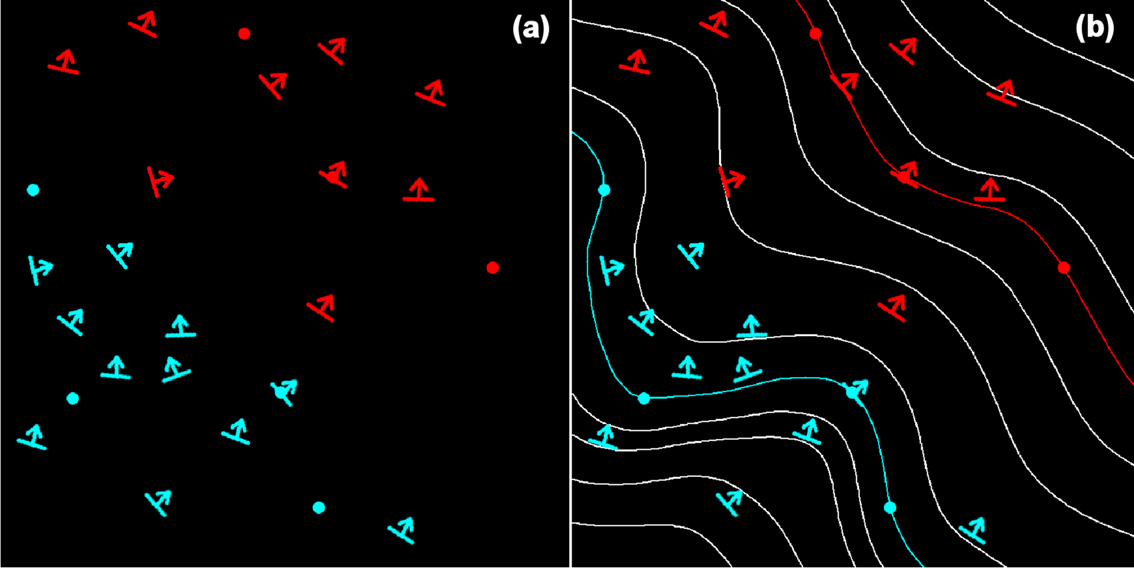
\includegraphics[width=1\textwidth]{Figures/calcagno_pot_field.png}
			\caption{woo a potential field! from \citet{calcagno2008geological}}\label{fig:pot_field}
		\end{figure}        
        Resulting potential fields can be used to describe geological interfaces as iso-surfaces in any kind of 3D geometry \citep{calcagno2008geological}. Fault geometries can be interpolated analogously. These can be infinite in the 3D space, interrelated in a fault network or finite. To account for the effect of faults on geological layers, discontinuous potential fields are created by applying discontinuous drift functions in the cokriging system. Additionally, geological rules allow for the representation of several types of interactions between sets of geological layers \citep{calcagno2008geological}.\\
        It is pointed out by \citet{calcagno2008geological}, that this method is particularly appropriate for cases in which knowledge about the geology is only given a sparse locations and is thus applicable for a wide variety of typical problem in geological settings. Its suitability for this work is furthermore emphasized by the possibility to modify the topology-defining geological pile to achieve different geometric realizations without altering the data. The model can thus be updated in the face of new data or interpretations \citep{calcagno2008geological}.
        
        \subsection{Economic significance and reservoir valuation}\label{sec:Reservoir_values}
        In this work, the generated structural models are to be assigned an economic significance in order to approach a real setting, in which hypothetical actors could have an interest in taking a decision, and thus, to evaluate the influence of the Bayesian inference of the decision-making process. Changes in Bayes actions are considered as a measure for this effect.\\
        For this purpose, it is assumed that a hydrocarbon reservoir system is represented by each geological model realization. These are typically comprised stratigraphically of at least one potential reservoir formation, succeeded by at least one sealing layer above. Additionally, a trapping mechanism is normally required (source?).\\
        The resulting reservoirs are to be valuated in a way that respective estimations on the basis of loss functions can be conducted, i.e. Bayesian decision theory is applicable. In the typical petroleum industrial setting, the main question is one of how much of the resource can be produced and how high the return on investment will be \citep{dean2007volumetric}.
        
        \subsubsection{Original oil-in-place and recoverable volumes as value measures}
        Before pressure and production tests have been conducted (i.e. before production has started), volumetric estimation is the only approach to assess the amount of hydrocarbons in place in a reservoir. From this value, recoverable reserves can be estimated based on an estimated recovery factor \citep{dean2007volumetric}.\\
        Oil-in-place and gas-in-place volumes are calculated based on:
        \begin{enumerate}
        \item Subsurface rock volume containing hydrocarbons. This is mainly defined by thickness and areal extend of the accumulation.
        \item Weighted average effective porosity of the reservoir rock.
        \item Water saturation in the reservoir rock.
        \item Hydrocarbon fluid properties \citep{dean2007volumetric}.
        \end{enumerate}
        As the cases used in this work are purely artificial, a pure oil accumulation is assumed. Using the factors listed above, the respective equation for original oil-in-place ($OOIP$) is formulated as follows:
        \begin{equation}\label{eq:OOIP}
        OOIP = A * h * \phi * (1 - S_W) * 1/FvF
        \end{equation}
        Where $OOIP$ is returned in $m³$. The hydrocarbon-filled rock volume is defined by the drainage area $A$ in $m²$ and the net pay thickness $h$ in $m$. Porosity $\phi$ and water saturation $S_W$ (interstitial water) are given in fraction of the rock volume. A dimensionless factor for the change in oil volume between reservoir conditions and standard conditions at surface is represented by the formation volume factor $FvF$. Thus, shrinkage of the oil volume brought to the surface is determined by $1/FvF$ \citep{dean2007volumetric}.\\
        Subsequently, the effectively recoverable oil volumes ($ROV$) can be calculated by multiplying the $OOIP$ with a recovery factor $RF$:
        \begin{equation}\label{eq:ROV}
                ROV = OOIP * RF = A * h * \phi * (1 - S_W) * 1/FvF * RF
        \end{equation}
        the recovery factor is influenced by a number of fluid properties, such as viscosity, density, solution oil/gas ratio and the formation volume factor. Thus, it is difficult to estimate \citep{dean2007volumetric}. Globally, the ultimate average recovery factor for oil fields is about 35\% \citep{labastie2011increasingRF}. For gas accumulations, however, recovery factors range typically between 70 and 90\% \citep{dean2007volumetric}.\\
        The models in this work are completely hypothetical and not based on real data. The inputs to these equations can thus be chosen arbitrarily to test the applied methods. However, to come to significant conclusion, it makes sense to utilize values that approximately represent real possible scenarios. Furthermore, as 3D geological structures are modeled here, the hydrocarbon-filled rock volume ($A * h$ in Equations \ref{eq:OOIP} and \ref{eq:ROV}) is defined by every realization of the uncertain geological model. The rock volume is thus an uncertain factor. Remaining factors can be implemented deterministically or as uncertain values, too. For most factors, it seems most suitable to define a normal distribution around a known typical value or global average, as it will return a high probability for common scenarios and occasionally produce cases of rare, more extreme values. (INSERT WHAT IS CHOSEN IN THE END - MAYBE MORE SENSE TO TAKE FIXED VALUES FOR THE FACTORS THEN RV, SO THAT ITS INFLUENCE IS CLEAR; THEN MAYBE INCLUDE POROSITY? OR COMPARE BOTH POSSIBILITIES?).\\
        Consequently, $OOIP$ and $ROV$ calculations represent the step following and using the results from computing the geological model, so that the realizations are assigned values that can be interpreted from a perspective of economic interest. The resulting values from numerous model runs are used as a base probability distribution for the true value, on which loss function estimation can be applied as described in Section \ref{sec:loss}. $OOIP$ and $ROV$ are applicable in a 3D setting, the 1D geological model introduced below in Section \ref{sec:1D_model}, however, requires the use of an abstract valuation system that is explained in Section \ref{sec:1D_score_system}.
        
        \subsubsection{Net present value}
        hmmm...
        
		\subsection{Numerical computational implementation via Python, GemPy and PyMC}
		Bayesian analysis can be conducted using probabilistic programming \citep{salvatier2016pymc3}. The implicit method of forward geological modeling, described above, is to be embedded in such a framework. For doing so, the programming language of choice in this work is Python. The merits of Python have been pointed out by \citet{behnel2010, salvatier2016pymc3, Langtangen2008}. Development is facilitated by an expressive but concise and clean syntax that is easy to learn. Python is dynamic, compatible with multiple platforms and offers good support for numerical computing. Integration of other scientific libraries and extension via C, C++, Fortran or Cython are easily possible \citep{behnel2010, salvatier2016pymc3, Langtangen2008}. Python is thus a straightforward tool for the implementation of central components of Bayesian analysis, such as custom statistical distributions and samplers \citep{salvatier2016pymc3}.\\
		The 3D geological modeling step in this work is implemented using GeMpy, an open-source, Python-based software that is able to generate and visualize complex 3D structural geological models based on the potential field interpolation method elaborated in Section \ref{sec:struc_geo_modeling} \citet{delaVarga2017gempy}. Its design allows for its application in a probabilistic setting, particularly by coupling it with PyMC (see below). At the time of writing this, GemPy is still under development (version 0.995), but is already functioning for the purpose of this work.\\
		For conducting the Bayesian analysis, GemPy is combined with the Python library PyMC, which was developed for conducting Bayesian inference and prediction problems in an open-source probabilistic programming framework \citep{davidson2015, salvatier2016pymc3}. Different model fitting techniques are provided in PyMC, such as the \textit{maximum a posteriori} (MAP) method and several (MCMC) sampling methods, including the Adaptive Metropolis explained in Section \ref{sec:mcmc} \citep{salvatier2016pymc3}. The components which are used to construct a statistical model, are represented by \textit{Deterministic} or \textit{Stochastic} variables in PyMC. the values of \textit{Deterministic} variables are completely dependent on its parents' values, as defined by a respective mathematical function \citep{salvatier2016pymc3}. \textit{Stochastic} variables are used to represent uncertain parameters $\theta$ or observed stochastic variables as likelihood functions $p(y|\theta)$ \citep{salvatier2016pymc3, delaVarga2016}. Complex mathematical relations between \textit{Stochastic} variables can be described through \textit{Deterministic} variables \citep{delaVarga2016}. Futhermore, PyMC allows for the creation of own object definitions inheriting from the class descriptions of these two variable types.\\		
		As of writing this, the newer PyMC3 is not yet supported by GemPy. Thus, it is resorted to PyMC 2 for 3D geological settings in this work. However, the newer PyMC 3 is used in a simple 1D scenario. \citet{salvatier2016pymc3} point out that the development of PyMC 3 is continuing, as the inclusion of further tools is planned for future updates.
		
		\section{Designing a case-specific loss function}\label{sec:LF_design}	
		As explained before in Section \ref{sec:loss}, the standard symmetric loss functions provide objectively good estimators minimizing expected loss by returning the median or mean respectively. However, assigning an economic notion to our model and assuming the case of an actor or decision maker in any field, naturally necessitates the consideration of preferences, interests and the overall subjective perspective such an individual or for example a company might have. Further constraints, properties and factors can also be specific to the field, industry or generally to the problem at hand. Consequently, the design of a more specific non-standard and possibly asymmetric loss function might be required, so that an adapted Bayesian estimator can be found. One that includes subjective aspects and difference in weighting of particular gains or losses, arising from an actor's inherent preferences and the environment in which the actor has to estimate or make a decision. In the face of several uncertain parameters, a perfectly true estimate is virtually unattainable. However, an attempt can be made to design a customized loss function that returns a Bayesian estimator involving the least bad consequences for an individual in a specific environment. Assuming the reservoir setting case and valuation methods introduced in Section \ref{sec:Reservoir_values}), such a customization attempt is made and explained step by step in the following. (SOURCES?)\\
		For the purpose of estimation, it makes sense that one of the standard loss functions is chosen as a basis and a customized loss function is developed from there. The absolute-error loss seems most appropriate for this case of hydrocarbon reservoir value estimation. Ideally, an actor would like to know the exact true value of interest, say the OOIP, so that investments or resources can be allocated appropriately in order to acquire economic gains. This allocation is the decision to be made or action to be taken. Deviations from the unknown true value in the form of over- and underestimation bring about an error and loss accordingly. In this case, it is assumed that investments increase linearly with linear growth in the value of the resource. For this reason, the absolute-error loss function is favored here over the squared-error loss function. It is chosen as the base function to which further development steps refer, based on mostly logical case-specific assumptions:
		
		\begin{enumerate}
			\item Step I: The standard symmetrical absolute-error loss function is chosen as a starting point for further customization steps:
			
			\begin{equation}
			L(\theta,\hat{\theta}) = |\theta - \hat{\theta}|
			\end{equation}  
			
			\item Step II: Considering the development of a hydrocarbon reservoir, it can be assumed that over-investing is worse than under-investing. Overestimating the size of an accumulation might for example lead to the installation of equipment or facilites that are actually redundant or unnecessary. This would come with additional unrecoverable expenditures. Consequences from underestimating, however, may presumably be easier to resolve. Additional equipment can often be installed later on. Hence, overestimation is weighted stronger in this loss function by multiplying the error with an overestimation factor \textit{a} (= 1.25):
			
			\begin{equation}\label{eq:LF_II}
			L(\theta,\hat{\theta}) = |(\theta-\hat{\theta})|*a
			\end{equation}
			
			\item Step III: The worst case for any project would be that its development is set into motion, expecting a gain, only to discover later that the value in the reservoir does not cover the costs of realizing the project, resulting in an overall loss. A petroleum system might also turn out to be a complete failure, containing no value at all, although the actor's estimate indicated the opposite. Here, this is referred to as worst case or fatal overestimation. A positive value is estimated, but the true value is zero or negative. This is worse than the "normal" non-fatal overestimation, where both values are positive and a net gain is still achieved, which is only smaller then the best possible gain of expecting the true value. Fatal overestimation is included in the loss function by using another weighting factor \textit{b} (= 2) that replaces \textit{a}:
			
			\begin{equation}\label{eq:LF_III}
			L(\theta,\hat{\theta}) = |(\theta-\hat{\theta})|*b
			\end{equation}
			
			(In other words: Fatal overestimation is twice as bad as simple underestimation.)
			
			\item Step IV: A worst case or fatal underestimation can also be derived from the idea of estimating a zero or negative value, when the true value is actually positive. This is assumed to be worse than non-fatal overestimation, but clearly better than fatal overestimation. No already owned resources are wasted, it is only the potential value that is lost, i.e. opportunity costs that arise from completely discarding a reservoir with a potential gain equal to the positive true value. Fatal underestimation is weighted using a third factor \textit{c}:
					
			\begin{equation}\label{eq:LF_IV}
			L(\theta,\hat{\theta}) = |(\theta-\hat{\theta})|*c
			\end{equation}
			
		\end{enumerate}
		
		Combining these adaption steps and the conditions defined in them, results in the following customized loss function:
		
		\begin{equation}\label{eq:LF_final}
		L(\theta,\hat{\theta}) =
		\begin{cases}
		|\theta - \hat{\theta}|, & \text{for } 0<\hat{\theta}<\theta  \\
		|\theta-\hat{\theta}|*a, & \text{for } 0<\theta<\hat{\theta} \\
		|\theta-\hat{\theta}|*b, & \text{for } \theta\leq0<\hat{\theta} \\
		|\theta-\hat{\theta}|*c, & \text{for } \hat{\theta}\leq0<\theta 
		\end{cases},
		\text{ with } a,b,c \in \mathbb{Q}
		\end{equation}  
		It is important to note that the weighting factors defined above can take basically any numerical values but should be chosen in a way that they appropriately represent the framework conditions of the problem. Here, based on the considerations named above, it is assumed that normal overestimation is 25\% (\textit{a} = 1.25), fatal overestimation 100\% (\textit{b} = 2) and fatal underestimation 50\% (\textit{c} = 1.5) worse than normal underestimation. \\		
		It has to be emphasized that this is just one possible proposal for loss function customization. There exists not one perfect design for such a case. Slight to strong changes can already be implemented by simply varying the values of the weighting factors \textit{a, b} and \textit{c}. Fundamentally different loss functions can also be based on a significantly different mathematical structure. Loss functions are customized regarding the problem environment and according to the to the subjective needs and objectives of an actor. Thus, they are mostly defined by the actor expressing his perspective. Changes in the individual's perception and viewpoint might lead to further customization needs even later on. (Especially considering individual persons as actors, psychological aspects may play a significant role.)
		
		(Estimate or prediction? True value only known if a "yes"-action (development) is taken.)
		INSERT PLOTS BASED ON EXAMPLE NORMAL FUNCTIONS?
		
		\subsection{Including different risk-affinities in the loss function}
		
		One can assume that several actors in one sector or decision environment may have the same general loss function, but different affinities concerning risks. This might be based for example on the different psychological factors or economic philosophies followed by companies. It might also be based on budgets and options such actors have available. An intuitive example is the comparison of a small and a large company. A certain false estimate or error might have a significantly stronger impact on a company which has a a generally lower market share and only few projects, than on a larger company which might possess a higher financial flexibility and for which one project is only one of many development options in a portfolio.
		
		In the following, the loss function is further adapted to consider different risk-affinities of several actors. Representing risk behavior in a loss function can also be done in different ways and regarding different types of risks. Here, bidding lower is considered the cautious, risk-averse option, as smaller losses can be expected from underestimating. Guessing higher is deemed riskier, as losses from overestimation are greater. However, bidding correctly on a higher value, will also return a greater gain. It is assumed that risk-friendly actors care less about fatal underestimation, i.e. they will rather develop a project than discard it. In the loss function, risk is simply included using a risk factor \textit{r} which alters the weighting factors \textit{a, b} and \textit{c} respectively:
		
		\begin{equation}\label{eq:LFR_final}
		L(\theta,\hat{\theta}) =
		\begin{cases}
		|\theta - \hat{\theta}|, & \text{for } 0<\hat{\theta}<\theta  \\
		|\theta-\hat{\theta}|*(a*r), & \text{for } 0<\theta<\hat{\theta} \\
		|\theta-\hat{\theta}|*(b*r), & \text{for } \theta\leq0<\hat{\theta} \\
		|\theta-\hat{\theta}|*(c*(r^{-0.5})), & \text{for } \hat{\theta}\leq0<\theta 
		\end{cases},
		\text{ with } a,b,c,r \in \mathbb{Q}
		\end{equation}
		
		According to this, for \textit{r} = 1 the risk-neutral loss function is returned, since \textit{a, b} and \textit{c} are not altered. For \textit{r} $<$ 1, the weight on overestimating is reduced and increased for fatal underestimation. This represents a more risk-friendly actor that is willing to bid on a higher estimate to attain a greater gain. For \textit{r} $>$ 1, the overestimation weight is increased in the loss function, the underestimation weight is decreased and respectively more risk-averse actors are prompted to bid on lower estimates.\\		
		The factor \textit{r} can take basically any positive values. However, since risk-neutrality is expressed by \textit{r} = 1, values 0 $<$ \textit{r} $<$ 2 are considered to be the most appropriate choices to represent both sides of risk-affinity equally here.		
		
		\section{1D geological reservoir modeling}\label{sec:1D_model}
		For simple understanding and a preliminary assessment of the Bayesian statistical methods and the loss function described above, they are first to be applied in the context of an abstract one-dimensional reservoir case. The underlying model and basic approach are inherited from \citet{delaVarga2016}. Parameters are adapted to more appropriately represent a reasonable geological petroleum system, consisting of a reservoir formation with overlying seal in the subsurface. In this 1D setting, only the interface depths and thicknesses of layers such as the reservoir or seal unit can be observed. Other defining aspects, such as structural entrapment, are assumed to be given. Limiting the model to only one dimension and a small number of uncertain stratigraphical parameters allows for a relatively straightforward and simplified approach to assessing an abstract type of value for a reservoir and using the custom loss function (Equation \ref{eq:LF_final}) for value estimation. The construction of the 1D geological model is described in the following.
		
			\subsection{Construction of the 1D geological model}\label{sec:1D_construction}	
			\citet{delaVarga2016} constructed a simple geological model using three uncertain positions in vertical one-dimensional space, marking hypothetical boundaries of layers in a subsurface column. The location probabilities for these points are defined by sampling from normal distributions. Standard deviations of these distributions increase with depth, representing an increase in uncertainty. For an approximate representation of a hydrocarbon reservoir system, the distribution means were set to depths of 2000 m (seal top), 2050 m (reservoir top) and 2200 m (reservoir bottom). STD-DEVIATIONS? These points confine two layers in the middle, from which the upper one can be labeled as seal and the lower one as reservoir. The resulting model with its possible layer boundary locations is illustrated in Figure \ref{fig:1D_model}.
		
			\begin{figure}[h]
				\centering
				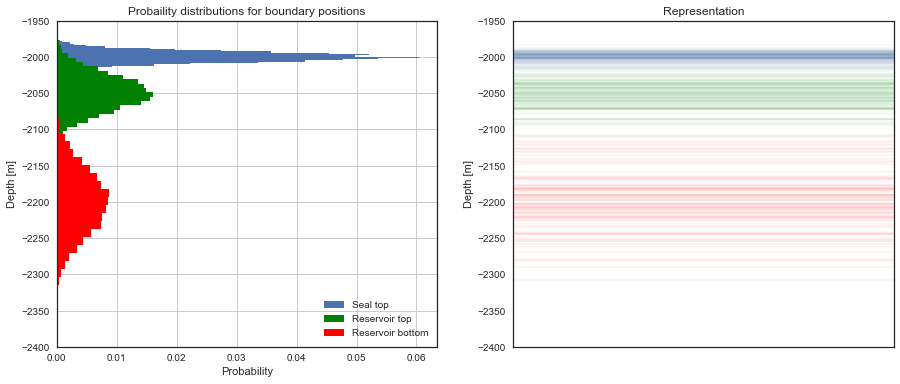
\includegraphics[width=1\textwidth]{Figures/1D_model.png}
				\caption{Probability distributions for positions of layer boundaries in the subsurface and a respective representation using lines.}\label{fig:1D_model}
			\end{figure}
		
	        \subsection{Abstract valuation (scoring) of the 1D geological model}\label{sec:1D_score_system}
	        For valuating a simplified 1D model, $OOIP$ and recoverable volume calculations are not applicable, as these require a 3D setting. Given only layer boundary positions in one vertical dimension, it is resorted to an abstract way of reservoir valuation by defining a scoring system. A dimensionless reservoir score is made dependent on three uncertain parameters which can be deduced from the 1D interface positions: (1) reservoir thickness, (2) reservoir top depth and (3) seal thickness (see Figure \ref{fig:3_parameters}).
	        	
	        \begin{figure}[h]
	        	\centering
	        	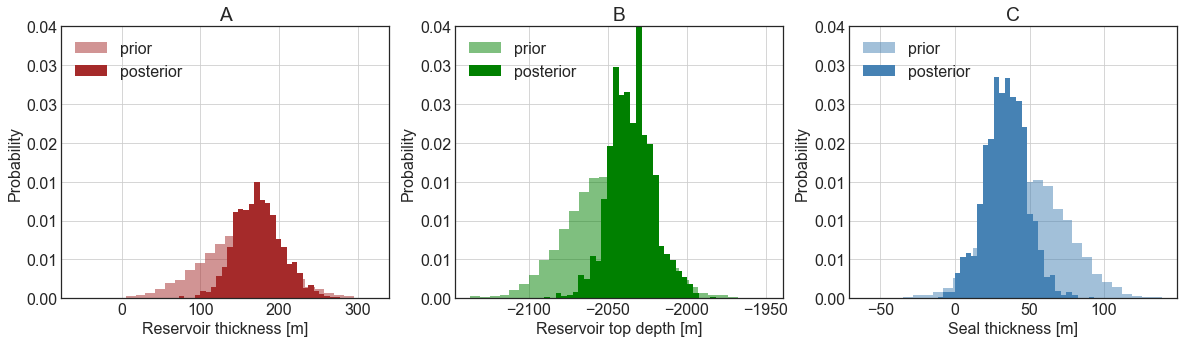
\includegraphics[width=1\textwidth]{Figures/3_parameters.png}
	        	\caption{Probability distributions for the three parameters deduced from the 1D model depicted in \ref{fig:1D_model}. Values from these parameter distributions are combined in \ref{eq:1D_score_system} attain a score to valuate reservoir model realizations.}\label{fig:3_parameters}
	        \end{figure}
	        
	        Assuming that reservoir thickness is a simplified indicator for the amount of extractable oil or gas and thus value in place, a gain in score can be correlated with increase in thickness. Here, two score points are assigned to one meter of thickness. Increasing costs of drilling are indicated by increasing depth of the reservoir top. Consequently, one negative score point is ascribed to every meter in depth. Samples from the probability distributions of these two parameters are drawn to model the true score of the reservoir (depth scores are subtracted from reservoir thickness scores).
	        A third parameter is defined by the seal thickness. Score points are not added or subtracted by this parameter directly. Instead, a threshold for seal reliability is defined beforehand. Here it is set at 20 m thickness. If the seal thickness falls below this threshold, it is assumed that the seal fails completely and thus all the potential value (positive score) of the reservoir is lost, while costs of depth (negative score) remain. Thus, a condition to check whether the seal is reliable is included in the model. A respective equation for the reservoir score $S_{res}$ is defined as follows:
			
			\begin{equation}\label{eq:1D_score_system}
			S_{res} = 
			\begin{cases}
			2h_{res} + d_{res}, & \text{for } h_{seal} >= 20  \\
			d_{res}, & \text{for } h_{seal} < 20
			\end{cases},
			\end{equation}
			
			Where reservoir thickness is given by $h_{res}$, seal thickness by $h_{seal}$ and reservoir depth, which is always a negative value, by $d_{res}$.
		
		\section{3D geological reservoir model}
		The concept of the 1D geological model is to be transferred and extended to a 3D setting that incorporates a more complete geological reservoir system. A three-dimensional space allows not only for better consideration of stratigraphical aspects, but also for the inclusion of structural formations, in particular reservoir trap-defining features.
		
		\subsection{Design of the 3D geological reservoir model}\label{sec:3D_design}
		For the purpose of exploring the effect of the methods of Bayesian analysis and decision theory in this work, the model is nevertheless to be kept relatively simple. Stratigraphically, it is designed to include one main reservoir unit (sandstone), one main seal unit (shale), an underlying basement through which hydrocarbon fluids could have flown upwards and overlying formations that are assumed to be permeable, so that hydrocarbons can leak upwards. Structurally, it is constructed to feature an anticlinal dome fold that is displaced by a normal fault. All layers are tilted so that they dip in the opposite direction of the fault plane dip. The original concept of this model is designed in a way, that a potential hydrocarbon trap is formed in the reservoir rock enclosed by the deformed seal and the normal fault.\\
		This trap is defined as the central feature of economic interest, more specifically, the trap volume. For conducting simple and straightforward volumetric calculations, it is assumed that defined safe traps are always "full-to-spill", i.e. the complete trap volume is hydrocarbon filled and the $OOIP$ is attained over this volume.
		
		- considering a petroleum production industry perspective, actors/ decision makers would be interested in the evaluation of value this potential reservoir
		- "traditionally", this is represented by volumetric calculations or estimations of the recoverable reserves
		- here: maximum volume of entrapment and subsequently, relative or hypothetical volumes of recoverable reserve can be calculated (for each model realization)
		- (later: numbers from example case are taken, to achieve estimations of the NPV for a development project realization)
		- looking at this structural model, not only the calculated volume can be taken into account, but also risk factors, such as fault permeabity seal safety (and capacity?), possible juxtapositions and leaks
		
		- as in the 1D case, uncertainties are introduced for a number of parameters in the model, in a way that they affect the resulting maximum volume of the trap (and following also the recoverable reserves)
		- again, a specific loss function is designed and applied on the results from numerous iterations of the constructed uncertain model, thus resembling the different value estimations/predictions or decisions different actors might make
		- (to bring this Bayesian method of using loss functions closer to the traditional application of deterministic decision-making in decision-trees, the continuous estimation space of the reservoir value (volume) is combined with the assumption, that the estimated value is linked to a consequent investment into a determined project development size. thus, the continuous approach is used to make the decision in a deterministic decision-making space. ))
		
		- later on,  the effect of adding information (in the form of likelihoods) is examined, particularly by looking at the changes in decision-making after applying this Bayesian updating and uncertainty has been reduced
		
		\subsection{Construction of the 3D geological reservoir model}\label{sec:3D_construction}
		- in the following, the construction and design of this model is described
		
		- base of the structural geological model is a 3Dcubic  space (block)  with 2000 m size in X, Y and Z x3
		- place layer positional points in three lines, resembling three hypothetical seismic lines as base information
		
		\subsection{Determination of the trap volume}
		
			\subsubsection{Finding spill and leak points}
			
			\subsubsection{Calculating the maximum trap volume}